\chapter{Esistenza del routing number}
\label{routing number}
È possibile andare a dimostrare che il valore di $rt(G)$ esiste sempre. Per compiere tale dimostrazione andiamo a compiere:
\begin{itemize}
    \item assumiamo che ci venga fornito $T$, un qualunque spanning tree del grafo $G$;
    \item cerchiamo un nodo foglia $u$ del grafo $T$;
    \item cerchiamo un nodo che abbia all'interno la pedina che ha come destinazione finale il nodo $u$, ovvero cerchiamo $v$ tale che $\pi(v) = u$;
    \item portiamo il nodo $v$ a destinazione $v$ scambiando a ogni passo i nodi, in modo che $P_v(\alpha) = \pi(v) = u$ dove $\alpha$ è il tempo finale; 
    \item una volta portato il nodo a destinazione, consideriamo ricorsivamente il grafo $T-\{u\}$; 
\end{itemize}

Per ottimizzare i tempi attuiamo due accorgimenti: 

\begin{itemize}
    \item La prima funzione necessaria è quella che riguarda il recupero di un nodo foglia. Per ottimizzare i tempi possiamo andare ad utilizzare una struttura dati ausiliaria, ad esempio uno stack, andiamo quindi a ordinare i nodi in base al loro grado e andiamo a inserirli in ordine inverso nello stack.
    In questo modo il primo elemento dello stack è sempre un nodo foglia. 
    Siccome i nodi di un grafo hanno un grado che può essere $[1,n-1]$ possiamo usare l'algoritmo di ordinamento \textit{counting sort} in modo da ordinare la coda in tempo lineare ($O(n)$). 
    A ogni iterazione estraiamo il primo elemento della coda (con un pop()), in modo che venga anche eliminato dalla coda in quanto "sistemato";
    \item Per ottimizzare il tempo che ci mettiamo a recuperare il nodo che ha come destinazione un nodo $u$, costruiamo un dizionario dove usiamo i nodi come indici e otteniamo per ogni nodo $u$ il nodo che contiene la pedina che deve trovarsi in quel nodo alla fine dell'algoritmo, cioè $v$ tale che $\pi(v)=u$.
    Supponiamo quindi che $dest[]$ sia un dizionario in modo tale da avere $dest[u]=v$.
    In questo modo il recupero di tale informazione ha un costo pari a $O(1)$. 
\end{itemize}

Definiamo, a tale scopo, lo pseudocodice per fare quanto appena descritto.

\begin{algorithm}
\caption{Calcolo del routing number su uno spanning tree $T$}\label{alg:cap}
\begin{algorithmic}[1]
\Require $T$: spanning tree di $G$, $dest$: mappa delle destinazioni finali, $foglie$: coda di nodi ordinata in base al grado dei nodi
\Ensure Numero totale di passi necessari (routing number)
\Function{routingNumber}{$T, foglie, dest$}
    \State $passi \gets 0$
    \If{$|V(T)| = 0$}
        \State \Return $passi$
    \Else
        \State $u \gets \text{foglie}.pop()$
        \State $v \gets \text{dest}[u]$
        \State $passi \gets \text{BFS\_modificato}(T, u, v)$
        \State $T \gets T - \{u\}$
        \State \Return $passi + \Call{routingNumber}{T, foglie, dest}$
    \EndIf
\EndFunction
\end{algorithmic}
\label{routing number spanning tree}
\end{algorithm}
\newpage
\begin{figure}[h]
    \begin{minipage}{0.5\textwidth}
        \centering
        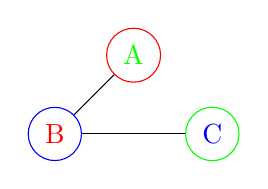
\begin{tikzpicture}
        \node[draw, circle, draw = blue, text = red] (B) at (0,0) {B};
        \node[draw, circle, draw = green, text = blue] (C) at (2,0) {C};
        \node[draw, circle, draw = red, text = green] (A) at (1,1) {A};
        
        % Edge
        \draw (A) -- (B);
        \draw (B) -- (C); 
        \end{tikzpicture}
        \caption{Disposizione iniziale del grafo T}
        \label{fig:inizio}
    \end{minipage}
    \hspace{0.05\textwidth}
        \begin{minipage}{0.5\textwidth}
        \centering
        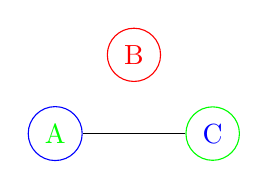
\begin{tikzpicture}
        \node[draw, circle, draw = blue, text = green] (B) at (0,0) {A};
        \node[draw, circle, draw = green, text = blue] (C) at (2,0) {C};
        \node[draw, circle, draw = red, text = red] (A) at (1,1) {B};
        
        % Edge
        \draw (B) -- (C); 
        \end{tikzpicture}
        \caption{Disposizione dopo il primo passo}
        \label{fig:primo passo}
    \end{minipage}
        \hspace{0.05\textwidth}
        \begin{minipage}{0.5\textwidth}
        \centering
        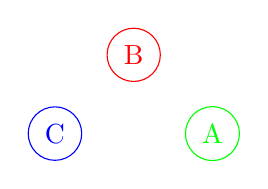
\begin{tikzpicture}
        \node[draw, circle, draw = blue, text = blue] (B) at (0,0) {C};
        \node[draw, circle, draw = green, text = green] (C) at (2,0) {A};
        \node[draw, circle, draw = red, text = red] (A) at (1,1) {B};
        \end{tikzpicture}
        \caption{Disposizione finale}
        \label{fig:finale}
    \end{minipage}
\renewcommand{\thefigure}{1}
\caption*{Esempio di funzionamento dell'algoritmo}
\end{figure}

\subsection{Funzioni ausiliarie}
Perché il tutto (\ref{routing number spanning tree}) funzioni, definiamo le funzioni ausiliarie.

\begin{algorithm}[h]
\caption{BFS Modificato per portare il nodo $v$ a destinazione $u$}
\small  % Riduce la dimensione del font
\begin{algorithmic}[1]
\Require $T$: grafo rappresentato con lista di adiacenza, $u$: nodo destinazione, $v$: nodo iniziale
\Ensure Numero di passi necessari per portare $v$ a $u$
\Function{BFS\_modificato}{$T, u, v$}
    \State $passi \gets 0$
    \State $coda \gets \text{Queue()}$
    \State $coda.\text{enqueue}(v)$
    \State $visitato \gets \text{Set()}$
    \While{$\text{coda is not empty}$}
        \State $nodo\_corrente \gets \text{coda.dequeue()}$
        \State $visitato.\text{add}(nodo\_corrente)$
        \If{$nodo\_corrente = u$}
            \State \Return $passi$
        \EndIf
        \ForAll{$w \in \text{Adj}(nodo\_corrente)$}
            \State $passi \gets passi + 1$
            \State $coda.\text{enqueue}(w)$
            \State $T \gets \text{swap}(T, nodo\_corrente, w)$
        \EndFor
    \EndWhile
\EndFunction
\end{algorithmic}
\end{algorithm}

\begin{algorithm}[h]
\caption{Funzione \textsc{swap} per scambiare le chiavi dei nodi}
\small  % Riduce la dimensione del font
\begin{algorithmic}[1]
\Require $T$: albero, $nodo\_corrente$: nodo corrente, $w$: nodo con cui scambiare la chiave
\Ensure Albero $T$ con chiavi scambiate
\Function{modificaAlbero}{$T, nodo\_corrente, w$}
    \State $temp \gets nodo\_corrente.\text{chiave}$
    \State $nodo\_corrente.\text{chiave} \gets w.\text{chiave}$
    \State $w.\text{chiave} \gets temp$
\EndFunction
\end{algorithmic}
\end{algorithm}

\section{Calcolo della Complessità}
L'algoritmo descritto \cite{routing number spanning tree} ha una complessità temporale che dipende dalla struttura del grafo e dal numero di nodi $n$. In particolare, possiamo calcolare la complessità come segue:

\begin{itemize}
    \item Il calcolo del routing number, che involve una BFS per ogni nodo, ha una complessità di $O(n + m)$, dove $n$ è il numero di nodi e $m$ il numero di archi nel grafo.
    \item In generale, il numero massimo di passi necessari per raggiungere la configurazione finale è di $O(n+m)$, poiché in ogni passo la ricerca di del nodo destinazione viene svolta in $O(1)$ dunque il costo dell'algoritmo equivale al costo della BFS sui nodi. 
\end{itemize}

Pertanto, la complessità complessiva dell'algoritmo è $O(n+m)$, dove $n$ è il numero di nodi nel grafo e $m$ è il numero di archi.